\chapter{Wavetable mit Modifier}


\begin{enumerate}[a)]
% a)
\item
Wählt man einen Gainwert von 0.9799, so erhält man ein innerhalb der drei Sekunden abklingendes Signal.
% b)
\item
Die drei erzeugten Signale klingen ähnlich, unterscheiden sich aber durch die Unterschiedlichen Amplitudenverhältnisse der Obertöne. Dadurch bekommt jeder Klang ein leicht unterschiedliches Timbre. Die Datei y\_4.wav klingt deswegen etwas heller als die Dateien y\_5.wav und y\_6.wav.
\begin{figure}[H]
    \center
    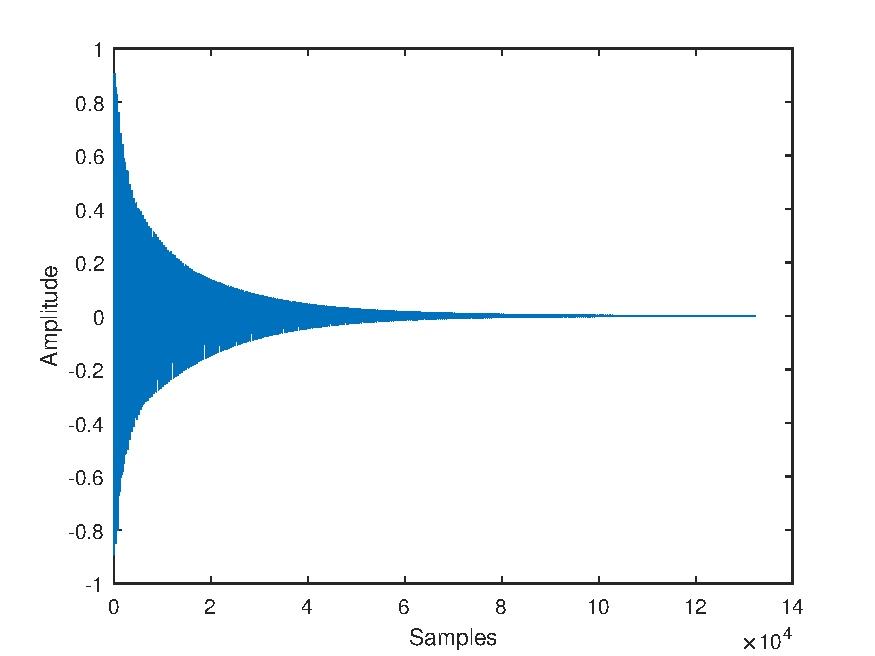
\includegraphics[width = 0.7\textwidth]{Figures/samples.pdf}
    \caption{Plot der Datei y\_4.wav}
    \label{fig:bs0}
\end{figure}

\newpage

% c)
\item
Die drei nachfolgenden Grafiken zeigen den Inhalt der Wavetable zu jeweils verschiedenen Zeitpunkten.

\begin{figure}[H]
    \center
    \includegraphics[width = 0.7\textwidth]{Figures/Anfang.pdf}
    \caption{Die Wavetable zu Beginn der Synthese.}
    \label{fig:wavetableBegin}
\end{figure}

In dieser Grafik ist die Wavetable in der ersten Iteration des Algorithmus zu sehen.
Das Signal hat einen stark rauschhaften Charakter.
Es lässt sich klar erkennen, dass der Ton aus einem weißen Rauschen generierte wurde. 

\begin{figure}[H]
    \center
    \includegraphics[width = 0.7\textwidth]{Figures/Mitte.pdf}
    \caption{Die Wavetable während der Synthese.}
    \label{fig:wavetableMiddle}
\end{figure}

Der zweite Plot wurde nach einigen wenigen Iterationen des Algorithmus erstellt.
Hier ist die Glättung, welche durch den gleitenden Mittelwert zu Stande kommt gut zu sehen.
Der rauschhafte Charakter des Signals ist verschwunden.
Die Wellenform erinnert nun eher an eine harmonische Schwingung.
Auch der Effekt des Gains ist bereits stark zu erkennen.
Die ursprüngliche Amplitude wurde deutlich abgeschwächt.

\begin{figure}[H]
    \center
    \includegraphics[width = 0.7\textwidth]{Figures/Ende.pdf}
    \caption{Die Wavetable gegen Ende der Synthese.}
    \label{fig:wavetableEnd}
\end{figure}

Der letzte Plot ist gegen Ende der 3 Sekunden aufgenommen.
Die Auswirkung des Gains ist hier klar zu erkennen. 
Das Signal ist deutlich abgeschwächt und klingt aus.

% d)
\item
Wir haben uns für drei Tiefpassfilter mit zunehmend höherer Dämpfung der hohen Frequenzanteile entschieden.
Dafür haben den gleitenden Mittwelwert über 5, 10 und 15 Samples gebildet um die Dateien y\_7.wav, y\_8.wav und y\_9.wav zu erzeugen.

% e)
\item
In der animierten Grafik, die beim Ausführen vom Matlabcode zu sehen ist, erkennt man das zeitliche Abklingen der Amplitude der Wellenform. 

\end{enumerate}
